% Shared preamble for the English summaries in this repository.
\documentclass[11pt,a4paper]{article}
\usepackage[margin=2.2cm]{geometry}
\usepackage[T1]{fontenc}
\usepackage[utf8]{inputenc}
\usepackage{lmodern}
\usepackage{amsmath,amssymb}
\usepackage{graphicx}
\usepackage{booktabs}
\usepackage{enumitem}
\usepackage[hidelinks]{hyperref}
\setlist{itemsep=2pt,topsep=4pt}
\setlength{\parindent}{0pt}
\setlength{\parskip}{5pt}
\graphicspath{{figures/}}
\newcommand{\summaryheader}[3]{%
  \begin{center}
    {\Large\bfseries #2}\\[3pt]
    {\large #1}\\[3pt]
    {\small Arshia Goshtasbi \textbullet{} MSc Electrical Engineering (Control), Iran University of Science and Technology \textbullet{} #3}
  \end{center}
  \vspace{2pt}\hrule\vspace{8pt}
  \noindent\textit{English summary of my original Persian report, which is kept as a PDF in this folder.}\par}

\begin{document}
\summaryheader{Convex Optimization, Comprehensive Homework}{Successive Convex Optimization, Facility Location, UAV Path Planning and an SDP}{Spring 1404 (2025)}

\section*{1. Successive convex optimization}
This is a local method for non-convex problems. Each step replaces the non-convex parts with convex approximations around the current point (linearisation or convex upper bounds), solves the convex problem, and repeats. It usually converges to a local optimum. A global optimum is guaranteed only under special structure, such as difference-of-convex problems with extra conditions.

\section*{2. Warehouse location as set covering}
For demand points $s_i$, candidate sites $d_j$ with build costs $c_j>0$, range $R$ and at most $k$ warehouses, I let $y_j\in\{0,1\}$ mean ``build at $d_j$'' and defined $N_i=\{j:\|d_j-s_i\|\le R\}$. The model is
\[
\min_y \sum_j c_jy_j \quad\text{s.t.}\quad \sum_{j\in N_i} y_j\ge 1\ \ \forall i,\qquad \sum_j y_j\le k .
\]

\section*{3. UAV path planning (\texttt{Q3.m})}
The cost is
\[
J=\sum_{t=0}^{T-1}\big(\|u_t\|^2+\alpha\|x_{t+1}-x_t\|^2\big)+\lambda\,R(x_0,\dots,x_T).
\]
It has double-integrator dynamics, box limits on velocity and acceleration, fixed start and goal, three circular obstacles and two linear danger zones. I compared hard obstacle constraints with a penalty approach. The circle constraints are linearised around the current path, each zone gets a slack variable penalised by $\lambda s^2$, and every iteration solves a QP with \texttt{quadprog} (linearise, solve, update with damping). The report runs three cases: $\lambda=0$ gives the straight, risky path, $\lambda=1$ a balanced one, and $\lambda=10$ a conservative one.

\textit{Re-running the script:} \texttt{quadprog} reports the linearised QP as infeasible at every iteration (exit flag $-2$), so the script falls back to its initial straight-line guess and all three curves coincide. I left the code as submitted.
\begin{center}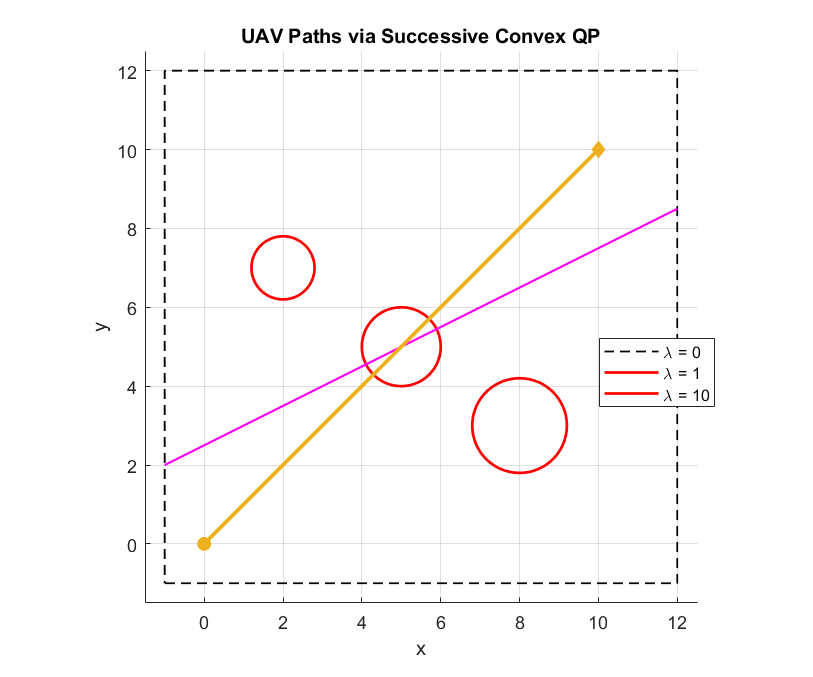
\includegraphics[width=0.5\linewidth]{Q3_1.png}\end{center}

\section*{4. A small SDP (\texttt{Q4.m}, CVX)}
The problem is $\min \operatorname{tr}(A^TX)$ s.t.\ $\operatorname{tr}(B^TXB)\ge\gamma$, $\operatorname{tr}(CX)\le\delta$, $X\succeq 0$. Its objective and constraints are linear in $X$ plus a PSD cone, so it is convex. I discussed the meaning of each constraint (a minimum controllability-type level and a bound on output variance) and the simplifications when $A$ is symmetric and $B$ is invertible. The report's solution satisfies $\operatorname{tr}(B^TXB)=1.5\ge\gamma$ and $\operatorname{tr}(CX)=0.4982\le\delta$, with eigenvalues of $X^\star$ equal to $0$ and $0.493$. The script needs CVX, which was not installed here, so it was not re-run.
\end{document}
